\subsection{Inter-Corporate Investments}

\begin{tabularx}{\textwidth}{p{5em}|p{10.5em}|X|X|p{9.5em}}
\hline
\rowcolor{gray!30}
 & Financial Assets & Associates & Business Combi & Joint Ventures \\
\hline
Influence & Not significant & Significant & Controlling & Shared Control \\
\hline
Interest \% & Usually $< 20\%$ & Usually $20\%$ to $50\%$ & Usually $>50\%$ or other indications of control & \\
\hline
Financial Reporting & Classified as
\xxx Fair value through profit or loss (FVPL)
\xxx Fair value through other comprehensive income (FVOCI)
\xxx Amortised Cost
& Equity Method
& Consolidation
& IFRS: Equity Method \\
\hline
IFRS & IFRS 9 & IAS 28 & IAS 27, IFRS 3, IFRS 10 & IFRS 11, IFRS 12, IAS 28 \\
\hline
GAAP & FASB ASC Topic 320 & FASB ASC Topic 323 & FASB ASC Topics 805 and 810 & FASB ASC Topic 323\\
\hline
\end{tabularx}
\begin{enumerate}[label=\roman*., before=\small]
\setlength{\itemsep}{0pt}
\item IFRS 9 Financial Instruments; IAS 28 Investments in Associates; IAS 27 Separate Financial Statements; IFRS 3 Business Combinations; IFRS 10 Consolidated Financial Statements; IFRS 11 Joint Arrangements; IFRS 12, Disclosure of Interests in Other Entities.
\item FASB ASC Topic 320 [Investments-Debt and Equity Securities]; FASB ASC Topic 323 [Investments- Equity Method and Joint Ventures]; FASB ASC Topics 805 [Business Combinations] and 810 [Consolidations].
\end{enumerate}

\subsubsection{Investment in Financial Assets: IFRS 9}

\begin{figure}[H]
\centering
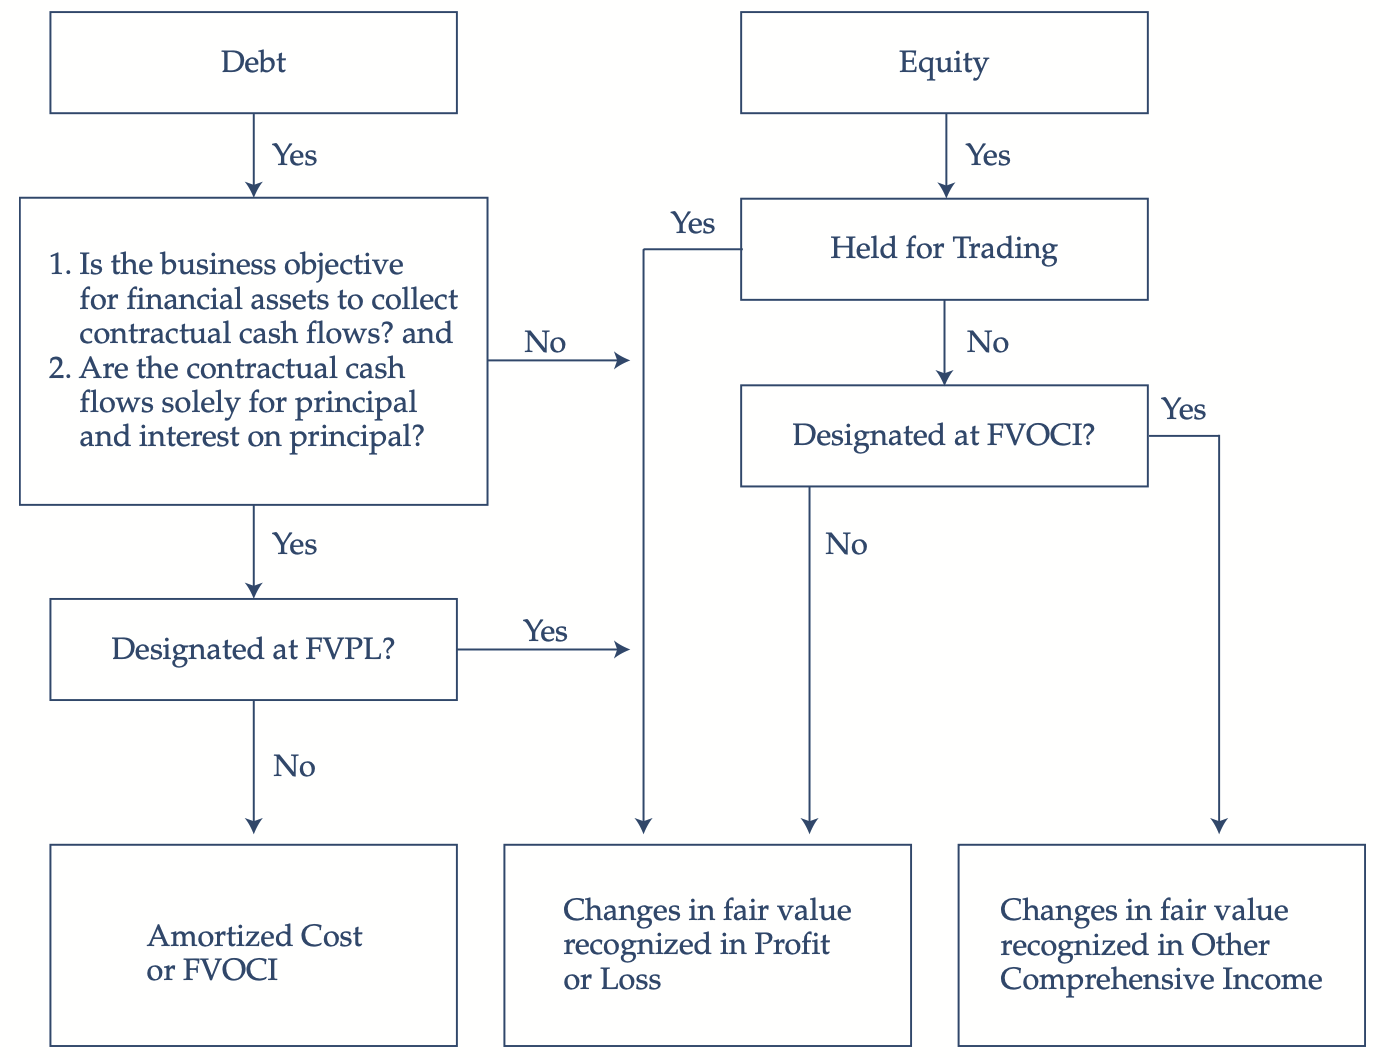
\includegraphics[scale=0.6]{fsa/ifrs9}
\caption{Financial Assets Classification and Measurement Model, IFRS9}
\end{figure}

\begin{definition} \hlt{Investment in Financial Assets: IFRS 9}\\
IFRS 9 considers contractual characteristics of cash flow and management of financial assets.\\
For loan impairment, expected credit loss model will be used.
\end{definition}

\begin{method} \hlt{Amortised Cost Method - Debt Only}\\
Debt securities meeting following two criteria are accounted for using the amortised cost method:
\begin{enumerate}[label=\roman*.]
\setlength{\itemsep}{0pt}
\item Business Model Test: debt securities are being held to collect contractual cash flows
\item Cash Flow Characteristics Test: the contractual cash flows are principal, or interest on principal, only.
\end{enumerate}
These are reported on the balance sheet at amortised cost - the original cost of debt plus or minus any discount or premium that has been amortised to date.\\
Interest income (coupon cash flow adjusted for amortisation of premium or discount) is recognised in income statement; subsequent changes in fair value are ignored.
\end{method}

\begin{method} \hlt{Fair Value through Profit or Loss - Debt and Equity}
\begin{enumerate}[label=\roman*.]
\setlength{\itemsep}{0pt}
\item Debt: classified as FVPL if held for trading, or if accounting for these securities at amortised cost results in accounting mismatch (inconsistency from different measurement bases for assets and liabilities)
\item Equity: classified as FVPL if held for trading. Otherwise, may be classified as either FVPL or FVOCI, choice is irrevocable.
\item Derivatives: classified as FVPL if not used for hedging. If asset has embedded derivative (i.e., convertible bonds), asset as a whole is valued at FVPL.
\end{enumerate}
Securities are reported on balance sheet at fair value. Changes in fair value (realised and unrealised) are recognised in income statement with any dividend or interest income.
\end{method}

\begin{method} \hlt{Fair Value through Other Comprehensive Income - Debt and Equity}\\
Securities are reported on balance sheet at fair value; any unrealised gain or loss is reported on OCI.\\
Realised gains or losses, dividends, interest income are reported on the income statement.
\end{method}

\begin{tabularx}{\textwidth}{p{5em}|p{14.5em}|X|p{16em}}
\hline
\rowcolor{gray!30}
 & Amortised Cost & FVPL & FVOCI \\
\hline
Balance Sheet & Amortised cost & Fair Value & Fair value, with unrealised gains and losses (GL) recognised in equity \\
\hline
Income Statement & Interest (including amortisation) & Interest & Interest \\
& & Dividends & Dividends \\
& Realised GL & Realised GL & Realised GL \\
& & Unrealised GL & \\
\hline
\end{tabularx}

\begin{method} \hlt{Reclassification under IFRS 9}
\begin{enumerate}[label=\roman*.]
\setlength{\itemsep}{0pt}
\item Debt: permitted only if business model has changed such that it significantly affects operations.
\item Equity: not permitted, as initial designation is irrevocable.
\end{enumerate}
\end{method}

\begin{method} \hlt{Loan Impairment under IFRS 9}\\
Incurred loss model for loan impairment replaced by expected credit loss model. Require companies to evaluate current and historical information on loan performance (loan commitments and lease receivables), and also forward-looking information.\\
Results in earlier recognition of loan impairment (12 month expected losses for performing loans, lifetime expected losses for non-performing loans).
\end{method}

\subsubsection{Investment in Associates: Equity Method}

\begin{remark} \hlt{Signs of Significant Influence}
\begin{enumerate}[label=\roman*.]
\setlength{\itemsep}{0pt}
\item Investment ownership between 20\% and 50\%
\item Representation on board of directors
\item Participation in the policy-making process
\item Material transactions between investor and investee
\item Interchange of managerial personnel
\item Technological dependency
\end{enumerate}
\end{remark}

\begin{method} \hlt{Equity Method}
\begin{enumerate}[label=\roman*.]
\setlength{\itemsep}{0pt}
\item Initial investment recorded at cost as non-current asset on BS.
\item Carrying amount of investment adjusted to recognise proportionate share of Profit and Loss (PnL); the PnL are recorded on IS.
\item Dividends and other distributions from investee is return of capital, reduce carrying amount of investment on BS, but not reported in investor PnL on IS.
\item On investee loss, investor will receive proportionate share of the loss, reducing the investment account, lower earnings in investor IS.
\item If investment value reduced to zero, equity method is discontinued; further losses will not be recorded. If investee subsequently reports profits, equity method is resumed after investor’s share of profit exceed the share of losses not recognised during the suspension period.
\end{enumerate}
GAAP: allows investments to be recorded at fair value.\\
IFRS: fair value option only available to VC, mutual funds, and similar entities. Decision to use fair value option is irrevocable; any changes in value (with dividends) recorded in income statement.
\end{method}
